\chapter{Návrh riešenia}

Pre použitie neurónových sietí v bežnej praxi doktorov pri diagnostike Alzheimerovej choroby je nevyhnutné, aby sa rozhodnutia neurónových sietí dali vysvetliť. Preto navrhujeme metódu na vyvsvetľovanie rozhodnutí neurónových sietí, ktorú overíme na MRI snímkach pri klasifikácii týchto snímok do dvoch skupín podľa diagnóz pacienta (CN, AD).

Vychádzajúc cieľa práce \textit{\ref{sec:goals_1} Vytvorenie novej alebo vylepšenie existujúcej metódy pre vysvetľovanie rozhodnutí neurónových sietí} navrhujeme metódu, ktorá vychádza z už existujúcej metódy \textit{RISE} (Sek. \ref{sec:rise}). Táto metóda dosiahla veľmi dobré výsledky oproti metódam GradCAM a LIME a považujem ju teda vhodný základ pre ďaľšie vylepšenia. Metóda RISE funguje na princípe zakrývania častí obrázka (tak ako iné perturbačné/oklúzne metódy) jednou hodnotou (tj. farbou). Po takomto prekrytí nevznikajú žiadné ostré hrany, ktoré by mohli neurónovú sieť mýliť ako u iných metódach, ktoré fungujú na princípe zakrývania častí obrazu.

Autori metódy RISE používali obrázky vo farebnom priestore RGB a prekrývali ich čiernou farbou (r = 0, g = 0, b = 0). MRI snímky nepoužívajú žiadnu farebnú schému, ale zachytávajú intenzitu (hodnoty sú zväčša reálne čísla). V tomto prípade môžeme zakrývať maximálnou alebo minimálnou hodnotou (minimálna hodnota je ekvivalentná RGB v prípade šedej). Toto zakrytie môže byť práve ďalším zdrojom zmätenia pre neurónovú sieť, keďže úbytky tkaniva sú vyjadrené nízkymi hodnotami na snímkoch.

Preto navrhujeme zakrývané miesta dokresliť určitou metódou spracovania obrazu (Sek. \ref{cap:image_processing}) alebo na zakrytie použiť inú hodnotu.
Pôvodná metóda bola ale narvhnutá pre obrázky (tj. 2D) a nie 3D volumetrické dáta, preto metódu RISEI upravujeme tak, aby vedela pracovať s 3D dátami - tj. budeme generovať 3D masky.

\section{RISEI \label{sec:risei}}

Metódu sme pomenovali \textit{Randomized Input Sampling for Explanation with Inpainting} (tj. náhodné vzorkovanie vstupu pre vysvetlovanie s dokreslovaním) so skratkou \text{RISEI}.

Keďže metóda vychádza už z existujúcej metódy, časť našej metódy je samozrejme rovnaká. Proces vytvorenia vysvetlenia klasifikácie (Obr. \ref{fig:risei_heatmap_generation}) do triedy $T$ pre obrázok $O$ modelom je teda nasledovný:

\begin{enumerate}
    \item Vytvorenie \textit{N} náhodne zamaskovaných obrázkov z obrázka $O$.
    \item Vloženie zamaskovaných obrázkov do modelu a následné získanie aktivácie pre triedu $T$.
    \item Vytvorenie a vizualizácia vysvetlenia pomocou tepelnej mapy.
\end{enumerate}

\begin{figure}[h!]
    \centering
    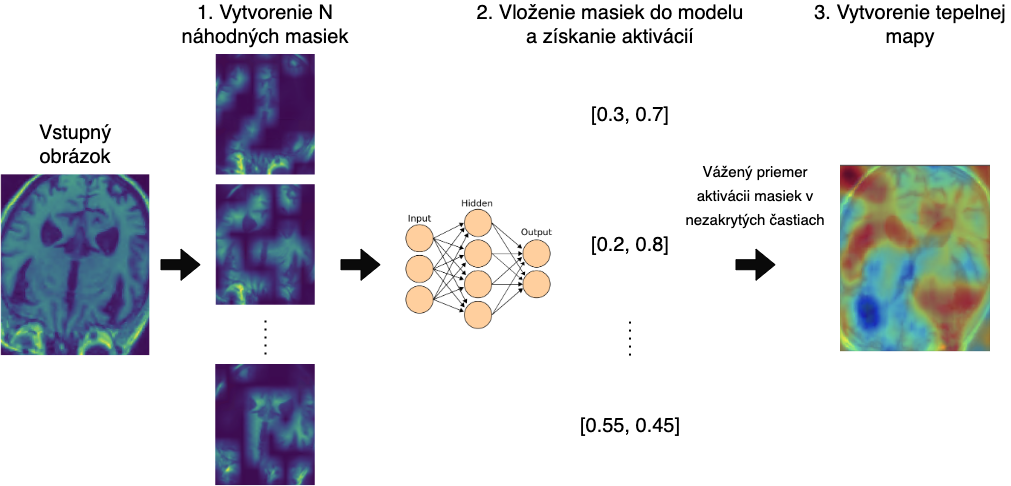
\includegraphics[scale=0.35]{assets/images/risei_heatmap_generation.png}
    \caption{Proces vysvetlenia klasifikácie - vytvorenia tepelnej mapy.}
    \label{fig:risei_heatmap_generation}
\end{figure}

Toto sú 3 hlavné kroky z ktorých pozostáva táto metóda, ďalej bližšie popíšeme jednotlivé z nich.

\subsection{Vytvorenie \textit{N} náhodne zamaskovaných obrázkov z obrázka \textit{O}}

Vytvorenie náhodne zamaskovaných obrázkov tiež pozostáva z niekoľkých krokov, pričom niektoré z nich môžu byť vykonávané paralelne. Tento krok sme znázornili diagramom (Obr. \ref{fig:risei_diagram}). Masky sa vytvárajú paralelne, pretože ''čierna'' maska ma jemné hrany a na dokreslenie potrebujeme naopak masku s ostrými hranami.

\begin{figure}[h!]
    \centering
    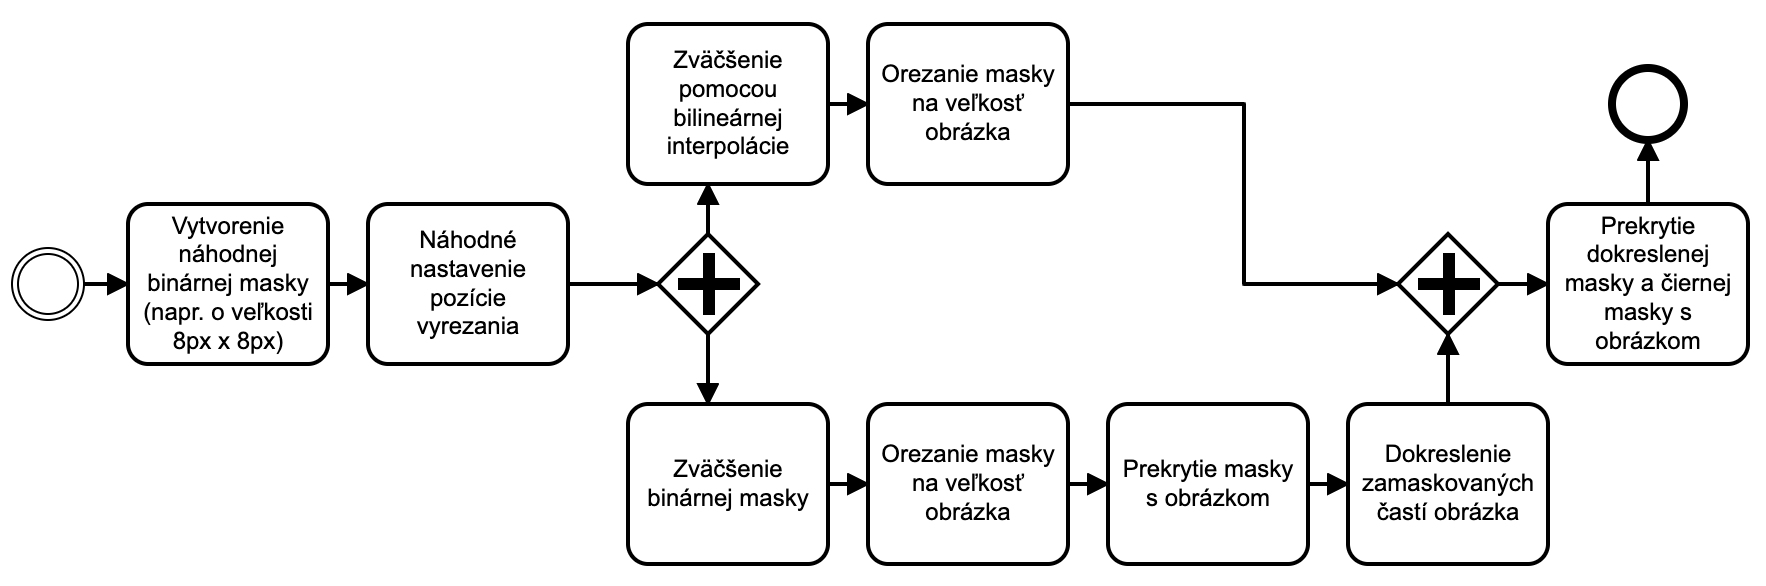
\includegraphics[scale=0.45]{assets/images/risei_diagram.png}
    \caption{BPMN diagram generovania jedného obrázka prekrytého maskou}
    \label{fig:risei_diagram}
\end{figure}

Oproti metóde \textit{RISE} vytvárame o jednu masku naviac, a teda je originálny obrázok prekrytý s viacerými maskami. Jednotlivé masky cez seba prekryjeme, pričom každej z nich nastavíme určité množstvo priehľadnosti. S týmto pomerom môžeme ďalej experimentovať a výsledky porovnávať. Môžeme porovnať použitie iba dokreslenej masky s iba ''čiernou'' maskou a tiež s použitím oboch v rôznych pomeroch.

Vytvorenie ''čiernej'' masky je rovnaké, ako pri metóde \textit{RISE}. Dokreslená maska vznikne dokreslením zakrytých (zamaskovaných) častí obrázka pomocou jedného z algoritmov na dokreslovanie (angl. inpainting). Tieto algoritmy sme popísali v sekcii \ref{cap:image_processing} Spracovanie obrazu. Obrázok \ref{fig:risei_inpainting_example} je príkladom dokreslenia častí vzorového obrázka na základe masky náhodne vygenerovanej masky (tento príklad je v 2D, naša metóda pracuje s 3D dátami).

Hodnota prekrytia môže byť akákoľvek konštanta - napríklad nula (hodnota v pôvodnej metóde RISE), jedna (maximálna hodnota v nami použitých dátach), stredná alebo priemerná hodnota zo snímky. Alebo prekrytie môže pozostávať viacero hodnôt na základe algoritmu - napr. dokreslenia.

\begin{figure}[h!]
    \centering
    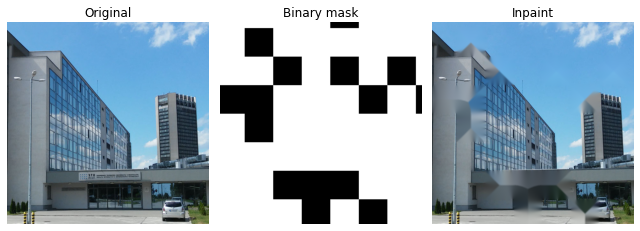
\includegraphics[width=13cm]{assets/images/risei_inpainting_example.png}
    \caption{Niektoré časti vzorového obrázoka (vľavo) boli dokreslené podľa náhodne vygenerovanej binárnej masky (v strede). Výsledný obrázok (vpravo) môže byť ešte prekrytý ''čiernou'' maskou s určitou priehľadnosťou.}
    \label{fig:risei_inpainting_example}
\end{figure}

\subsection{Vloženie zamaskovaných obrázkov do modelu a následné získanie aktivácie pre triedu \textit{T}.}

Krok vloženia zamaskovaných obrázkov do modelu je identický s originálnou metódou \textit{RISE}. Zamaskované obrázky sú vložené do modelu, metóda následne zozbiera výsledné aktivácie pre triedu, pre ktorú ju tepelná mapa vytváraná - vytvárame takú tepelnú mapu, ktorá hovorí, ktoré oblasti obrázka sú viac/menej dôležité pre vybranú triedu.

\subsection{Vytvorenie a vizualizácia vysvetlenia pomocou tepelnej mapy.}

Tento krok je identický s originálnou metódou \textit{RISE}. Nasledovný vzorec \ref{eq:risei_heatmap_1} vyjadruje výpočet dôležitosti $I$ pre každý voxel $[x, y, z]$ snímky, kde $n$ je počet všetkých zamaskovaných snímok. Funkcia $p(k, x, y, z)$ vracia vracia predikciu (tj. aktiváciu v kontexte neurónových sietí) pre predikovanú triedu (v prípade binárnej klasifikácie) z modelu pre zamaskovanú snímku $k$. Funkcia $c(k, x, y, z)$ vracia mieru zakrytia/dokreslenia maskou, pričom $H(c) = <0, 1>$, kde $1$ znamená úplné prekrytie/dokreslenie a $0$ žiadne prekrytie/dokreslenie. Rovnako, ako metóde \textit{RISE}, počítame vážený priemer.

\begin{equation} 
    I_{x, y, z} = \frac{\sum_{k}^{n} p(k, x, y, z) * (1 - c(k, x, y, z))}{\sum_{k}^{n} p(k, x, y, z)}
    \label{eq:risei_heatmap_1}
\end{equation}

Navrhovaná metóda do orignálnej metódy pridáva niekoľko parametrov a najmä výpočtovo náročné dokresľovanie, preto bude nutné nájsť vhodné nastavenie parametrov, aby výpočet vysvetlenia nebol príliš časovo náročný. Práve výpočtová náročnosť môže byť jednou zo slabín tejto metódy. Takisto aj samotná dokreslená časť obrázka môže byť príčinou zmätenia neurónovej siete.

\section{Overenie riešenia \label{sec:evaluation_design}}

Našu metódu v prvom rade porovnávame s originálnou metódou RISE (tj. či sa nám podarilo vytvoriť lepšiu metódu) a následne s inou existujúcou metódou (LRP, GradCAM, Guided Backprop alebo Guided GradCAM). Z týchto metód je najviac vhodná metóda LRP, keďže už bolo jej použitie pri vysvetľovaní rozhodnutí neurónových sietí detegujúcich Alzheimerovu chorobu (Sekcia \ref{sec:ad_nn_explanation}) skúmané. Tieto experimenty vykonávame na CN a AD vzorkách. Sledujeme kvalitu navrhnutej metódy (oproti ostatným metódam) a na základe týchto tepelných máp vyhodnocujeme mieru správnosti modelu.

\subsection{Dátová sada} Experimenty budeme vykonávať na dátovej sade ADNI, ktorá obsahuje MRI snímky AD pacientov. Táto dátová sada bola použitá aj na trénovanie state-of-the-art modelu na diagnsotiku Alzheimerovej choroby \cite{esmaeilzadeh2018end}, ale aj pri vysvetľovaní rozhodnutí neurónovej siete pomocou LRP \cite{bohle2019layer}. 

% Na tejto dátovej sade budeme musieť vykonať rovnaké predspracovanie ako \citeauthor*{bohle2019layer}, aby sme sa s ich výsledkami mohli porovnať. Prípadne môžeme vykonať vlastné predspracovanie, ale budeme musieť vykonať aj experimenty s metódou LRP.

\section{Model \label{sec:design_model}}

Na vytváranie tepelmých máp je nevyhnutný model. Navrhnutú metódu porovnávame na niekoľkých modeloch - architektúrach neurónových sietí. Z nich vyberieme najvhodnejší pre ďaľšie detailnejšie experimenty.

\begin{itemize}
    \item \textbf{3D konvolučná neurónová sieť od \citeauthor*{esmaeilzadeh2018end}} Túto neurónovú sieť sme vybrali, pretože jej autori pomocou nej dosiahli veľmi dobré výsledky (94.1\% presnosť).
    \item \textbf{2D ResNet a 3D ResNet} Keďže reziduálne neúronové siete dosahujú pri klasifikačných úlohách nad obrazovými dátami veľmi dobre výsledky použijeme aj tieto architektúry.
\end{itemize}

Do týchto neurónových sietí sme ešte pridávame dropout a dávkovú normalizáciu (angl. batch normalization). Dropout pridávame pred plne prepojené vrstvy. Dávkovú normalizáciu pridávame v konvolučných vrstvách pred aplikovaním nelinearity, tak ako je to odporučené od \citeauthor*{ioffe2015batch} v \textit{Batch Normalization: Accelerating Deep Network Training by Reducing Internal Covariate Shift}. Na poslednej vrstve používame dva neuróny s aktivačnou funkciou \textit{softmax}.

Snímky s dátovej sady sme sa rozhodli augmentovať (Obr. \ref{fig:augmentations}) s cieľom zväčšenia počtu rôznych pozorovaní. Dáta náhodne augmentujeme v každej dávke (angl. batch). Používame nasledovné augmentácie:

\begin{itemize}
    \item Vymenenie hemisfér mozgu (\citeauthor*{esmaeilzadeh2018end} \cite{esmaeilzadeh2018end}) s pravdepodobnosťou 50\%
    \item Náhodná rotácia o 0 až 5 stupňov s pravdepodobnosťou 20\%
    \item Náhodné priblíženie do 80\% veľkosti snímku s pravdepodobnosťou 20\%
    \item Náhodné gaussovské rozmazanie (max $sigma = <0.85, 1>$) s pravdepodobnosťou 20\%
    \item Náhodný gaussovský šum pravdepodobnosťou 20\%
\end{itemize}

\begin{figure}[H]
    \centering
    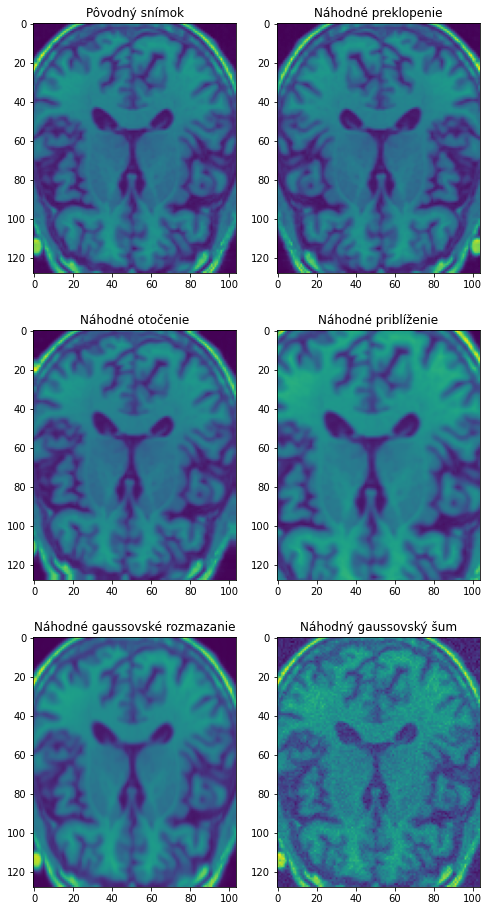
\includegraphics[width=10cm]{assets/images/augmentations.png}
    \caption{Príklady aplikácie augmentácií.}
    \label{fig:augmentations}
\end{figure}


\subsection{Experimenty \label{sec:design_experiments}}

Najskôr vyhodnocujeme nami navrhnutú metódu pomocou sledovania kvality tepelných máp. Následne overujeme správnosť modelu pomocou nami navrhnutej metódy, avšak je nutné, aby metóda generovala kavlitné tepelné mapy.

\subsubsection{Určenie kvality metódy vysvetľovania rozhodnutí modelu \label{sec:evaluation_design_method_quality}}

Kvalitu metódy vysvetľovania rozhodnutí modelu sledujeme určovaním kvality tepelnej mapy. Tá v kontexte našej práce hovorí o tom, do akej miery táto mapa odzrkadľuje to, na základe čoho sa model rozhoduje. Toto budeme merať metrikami \textit{insertion (AUC)} a \textit{deletion (AUC)}, ktoré sme bližšie popísali v sekcii \ref{sec:rise}. Tieto metriky nám povedia, aká dobrá je naša metóda na vysvetľovanie.

Keďže naša metóda generuje tepelné mapy pomocou vygenerovania veľkého množstva náhodných masiek, je vhodné skúmať, ako sú tieto tepelné mapy konzistentné pri niekoľkých použitiach metódy rovnakom MRI snímku. Konzistentnosť máp môžeme merať pomocou podobnosti medzi jednotlivými tepelnými mapami vygenerovaními pre tú istú snímku a ten istý model (napr. ako súčet absolútných hodnôt rozdielov medzi voxelmi v oboch tepelných mapách). Čím je táto podobnosť väčšia, tým je metóda pri generovaní máp viac konzistentná.

\subsubsection{Určenie správnosti modelu \label{sec:heat_maps_and_model_segmentation_masks}}

Správnosť modelu sme určujeme na na základe tepelných máp vytvorených pomocou metódy na vysvetľovanie predikcií modelu. Overujeme do akej miery dávajú tepelné mapy zmysel v kontexte skutočnej anatómie mozgu, tj. či tepelná mapa pre správnu predikciu ukazuje na klinicky relevantné oblasti mozgu. Sledujeme, či tepelná mapa nehovorí o tom, že sa model rozhodol na základe takej oblasti mozgu, z ktorej sa Alzheimerova choroba nedá zistiť. Veľkú úlohu pri určovaní správnosti modelu zohráva aj kvalita natrénovaného modelu, tú môžeme merať pomocou metrík z práce od \citeauthor*{bohle2019layer} v ktorej sa autori zaoberali vyhodnocovaním tepelných máp vypočítaných pomocou metódy LRP. Tieto metriky sú nasledovné (relevancia je v našom prípade teplota na tepelnej mape):

\begin{itemize}
    \item súčet relevancie v jednotlivých častiach mozgu (podľa segmentačných masiek) pre AD a CN
    \item hustota relevancie v jednotlivých častiach mozgu (podľa segmentačných masiek) pre AD a CN, berie ohľad na veľkosť danej časti mozgu
    \item prírastok relevancie v jednotlivích častiach mozgu (podľa segmentačných masiek) vypočítaný ako pomer priemernej relevancie každej triedy v danej časti mozgu
\end{itemize}

\section{Zhrnutie}

V tejto kapitole sme navrhli metódu na vysvetľovanie rozhodnutí modelov strojového učenia a spôsob jej implementácie. Navrhnutú metódu budeme overovať na neurónových sieťach detegujúcich Alzheimerovu chorobu s cieľom odhaľovania nesprávnych rozhodnutí.
